\documentclass[a4paper, 12pt]{article}
\usepackage[utf8]{inputenc}
\usepackage[left=1.5cm,text={17cm, 26cm},top=1.5cm]{geometry}
\usepackage[czech]{babel}
\usepackage{float}
\usepackage{graphicx}
\usepackage{keystroke}
\usepackage{menukeys}
\linespread{1.3}
\usepackage{enumitem}
\setlist[1]{itemsep=-5pt}
\begin{document}

\thispagestyle{empty}
\begin{minipage}[b]{0.5\textwidth}
{\fontsize{18pt}{10pt}\selectfont\underline{Uživatelská příručka}}\\[4mm]
{\fontsize{150pt}{150pt}\selectfont\textbf{Alp(h)acalc}}\\[2mm]
{\fontsize{10pt}{10pt}v1.0 Absinthe}\\
\newline
\newline
\newline
\newline
\newline
\newline
\newline
\newline
\newline
\newline
{\fontsize{12pt}{10pt}\selectfont\textit{Děkujeme, že jste si vybrali právě\\ náš Apl(h)acalc.}}\\
%\newline
\phantom{xxxxxxxx} {\fontsize{12pt}{10pt}\selectfont\textit{Vaši xhlava52, xkraus13, xvuthi00}}\\
\end{minipage}%
\begin{minipage}[b]{0.07\textwidth}
\begin{figure}[H]
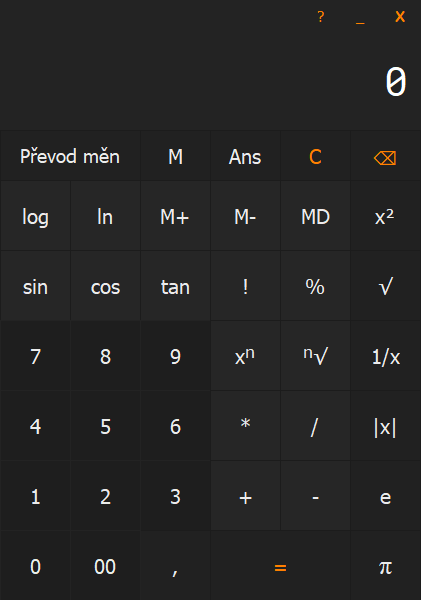
\includegraphics[scale=0.6]{kalkulacka.png}
\end{figure}
\end{minipage}
\newline

\tableofcontents
\newpage
\section{Instalace a odinstalace}
    \subsection{Automaticky}
        \subsubsection{Instalace}
            \begin{enumerate}
                \item Stáhněte si DEB instalační balíček z https://github.com/jakubhlava/alphacalc/releases (nebo si jej zkompilujte ze zdrojových kódů - viz níže)
                \item Běžným způsobem jej nainstalujte dle možností vaší Linuxové distribuce
                    \begin{enumerate}
                        \item Pomocí \texttt{apt} příkazem \texttt{apt install cesta/k/balíčku}
                        \item V Ubuntu lze pro instalaci a odinstalaci využít Software Center
                    \end{enumerate}
                \item Spusťte z menu vašeho OS nebo příkazem \texttt{alphacalc} v terminálu
            \end{enumerate}
        \subsubsection{Odinstalace}
            \begin{enumerate}
                \item Běžným způsobem odinstalujte balíček
                \begin{enumerate}
                    \item Pomocí \texttt{apt} příkazem \texttt{apt remove alphacalc}
                    \item Ze seznamu nainstalovaných aplikací v Ubuntu Software Center
                \end{enumerate}
            \end{enumerate}
    \subsection{Manuálně}
        \subsubsection{Instalace ze zdrojových kódů}
            \begin{enumerate}
                \item Z webu nebo pomocí příkazu \texttt{git}, pokud jej máte v systému nainstalovaný si naklonujte repozitář https://github.com/jakubhlava/alphacalc/
                \item Ručně podle seznamu v README repozitáře nebo automaticky pomocí \texttt{make prerequisites} si nainstalujte vývojové závislosti aplikace
                \item Zkompilujte instalační balíček pomocí příkazu \texttt{make all}
                \item Pokud chcete instalovat pomocí DEB balíčku, postupujte podle návodu k automatické instalaci (a poté i odinstalaci), jinak pokračujte dále
                \item Ve složce \texttt{build} v kořenové složce repozitáře se nachází soubor \texttt{AlphaCalc-x.y.tar.gz}, kde \texttt{x.y} značí verzi, tento balíček je možno nainstalovat ve složce \texttt{build} pomocí příkazu \texttt{pip3 install ./AlphaCalc-x.y.tar.gz}
                \item V případě, že požadujete ikonu v menu vašeho operačního systému:
                \begin{enumerate}
                \item Zkopírujte soubor \texttt{src/buildfiles/icons/alphacalc.desktop} \\
                do složky \texttt{/usr/share/applications}
                \item Zkopírujte soubor \texttt{src/buildfiles/icons/alphacalc.png} \\
                do složky \texttt{/usr/share/icons}
                \item Ikonu vytvořte příkazem \texttt{xdg-desktop-menu install --novendor \\
                 /usr/share/applications/alphacalc.desktop}
                \end{enumerate}
            \end{enumerate}
        \subsubsection{Instalace z PIP balíčku}
            \begin{enumerate}
                \item Stáhněte si balíček pro PIP z https://github.com/jakubhlava/alphacalc/releases/ (soubor \texttt{AlphaCalc-x.y.tar.gz})
                \item Nainstalujte si minimální závislosti (Python3 a pip) příkazem \\
                        \texttt{apt install python3 python3-pip}
                \item Příkazem \texttt{pip3 install ./AlphaCalc-x.y.tar.gz} ve složce se staženým balíčkem, kde \texttt{x.y} je verze balíčku nainstalujete balíček vč. závislostí
                \item V případě, že požadujete ikonu v menu vašeho operačního systému, pokračujte podle návodu výše v části \textbf{Instalace ze zdrojových kódů}
            \end{enumerate}
        \subsubsection{Odinstalace PIP balíčku}
            \begin{enumerate}
                \item Pokud jste při instalaci vytvářeli ikonu v menu postupujte při odstranění takto:
                    \begin{enumerate}
                        \item Vymažte ikonu příkazem \texttt{xdg-desktop-menu uninstall --novendor \\
                        /usr/share/applications/alphacalc.desktop}
                        \item Vymažte soubor \texttt{/usr/share/applications/alphacalc.desktop}
                        \item Vymažte soubor \texttt{/usr/share/icons/alphacalc.png}
                    \end{enumerate}
                \item Odinstalujte balíček kalkulačky příkazem \texttt{pip3 uninstall alphacalc}
                \item Volitelně můžete odinstalovat i závislosti balíčku \texttt{alphacalc} příkazem \texttt{pip3 uninstall pyside2 requests}
            \end{enumerate}

    \subsection{Možné problémy při instalaci}
    \begin{itemize}
        \item Příkaz \texttt{pip3} neexistuje. \\ \textit{ŘEŠENÍ: místo příkazu pip3 použijte příkaz \texttt{python3 -m pip}}
        \item Příkaz \texttt{...} neexistuje. \\ \textit{ŘEŠENÍ: zkontrolujte, zda máte nainstalovány všechny závislosti dle README}
        \item Nedaří se vám vytvořit ikona. \\ \textit{ŘEŠENÍ: zkontrolujte, zda vám v systému nechybí balíček \texttt{xdg-utils} a zda je s ním váš desktop kompatibilní} 
    \end{itemize}
                
                
        
                
%\newpage
\section{Ovládání pomocí klávesnice}
Pomocí klávesnice můžeme zadávat čísla, desetinnou čárku a základní početní operace jako: \keys{{+}}, \keys{{-}}, \keys{{*}}, \keys{{/}}. \\
Výsledek zobrazíme stisknutím kterékoli klávesy: \keys{\return}.\\
\keys{\backspace} mažeme po jednotlivých číslicích.\\
\keys{\delname} smažeme celé zobrazené číslo a také počítaný příklad.

\section{Funkce}
%+
\begin{minipage}{0.07\textwidth}
\begin{figure}[H]

\includegraphics[scale=0.7]{plus.jpg}
\end{figure}
\end{minipage}
\begin{minipage}{0.45\textwidth}
\begin{itemize}
\item sečte dvě čísla
\item $x$\ \keys{{+}}\ $y$ \keys{=}
\end{itemize}
\end{minipage} %
\begin{minipage}{0.07\textwidth}
\begin{figure}[H]

\includegraphics[scale=0.7]{minus.jpg}
\end{figure}
\end{minipage}
\begin{minipage}{0.45\textwidth}
\begin{itemize}
\item odečtě dvě čísla
\item $x$ \keys{{-}} $y$ \keys{=}
\end{itemize}
\end{minipage}
\\%*
\begin{minipage}{0.07\textwidth}
\begin{figure}[H]

\includegraphics[scale=0.7]{mul.jpg}
\end{figure}
\end{minipage}
\begin{minipage}{0.45\textwidth}
\begin{itemize}
\item vynásobí dvě čísla
\item $x$ \keys{*} $y$ \keys{=}
\end{itemize}
\end{minipage} %
\begin{minipage}{0.07\textwidth}
\begin{figure}[H]
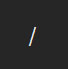
\includegraphics[scale=0.7]{div.jpg}
\end{figure}
\end{minipage}
\begin{minipage}{0.45\textwidth}
\begin{itemize}
\item vydělí dvě čísla
\item $x$  \keys{{/}}  $y$ \keys{=}
\end{itemize}
\end{minipage}
\\%xn
\begin{minipage}{0.07\textwidth}
\begin{figure}[H]
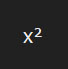
\includegraphics[scale=0.7]{x2.jpg}
\end{figure}
\end{minipage}
\begin{minipage}{0.45\textwidth}
\begin{itemize}
\item umocní číslo na druhou
\item $x$ \keys{{$x^2$}}
\end{itemize}
\end{minipage}
\begin{minipage}{0.07\textwidth}
\begin{figure}[H]
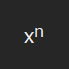
\includegraphics[scale=0.7]{xn.jpg}
\end{figure}
\end{minipage}
\begin{minipage}{0.45\textwidth}
\begin{itemize}
\item umocní číslo $x$ na $n$
\item $x$ \keys{$x^n$} $n$ \keys{=}
\end{itemize}
\end{minipage}
\\%v
\begin{minipage}{0.07\textwidth}
\begin{figure}[H]
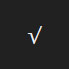
\includegraphics[scale=0.7]{v.jpg}
\end{figure}
\end{minipage}
\begin{minipage}{0.45\textwidth}
\begin{itemize}
\item vypočítá druhou odmocninu čísla
\item \keys{$\sqrt{\phantom{x}}$} $x$ \keys{=}
\end{itemize}
\end{minipage}
\begin{minipage}{0.07\textwidth}
\begin{figure}[H]
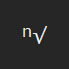
\includegraphics[scale=0.7]{nv.jpg}
\end{figure}
\end{minipage}
\begin{minipage}{0.45\textwidth}
\begin{itemize}
\item vypočítá $n$ odmocninu čísla
\item $n$ \keys{$\sqrt[n]{\phantom{x}}$} $x$ \keys{=}
\end{itemize}
\end{minipage}
\\%abs
\begin{minipage}{0.07\textwidth}
\begin{figure}[H]

\includegraphics[scale=0.7]{abs.jpg}
\end{figure}
\end{minipage}
\begin{minipage}{0.45\textwidth}
\begin{itemize}
\item spočítá absolutní hodnotu čísla
\item $x$ \keys{$|x|$}
\end{itemize}
\end{minipage}
\begin{minipage}{0.07\textwidth}
\begin{figure}[H]
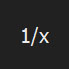
\includegraphics[scale=0.7]{1x.jpg}
\end{figure}
\end{minipage}
\begin{minipage}{0.45\textwidth}
\begin{itemize}
\item spočítá převrácenou hodnotu čísla
\item  $x$ \keys{$1/x$}
\end{itemize}
\end{minipage}
\\%fac
\begin{minipage}{0.07\textwidth}
\begin{figure}[H]

\includegraphics[scale=0.7]{fac.jpg}
\end{figure}
\end{minipage}
\begin{minipage}{0.45\textwidth}
\begin{itemize}
\item vypočítá faktoriál čísla
\item $x$ \keys{!}
\end{itemize}
\end{minipage}
\begin{minipage}{0.07\textwidth}
\begin{figure}[H]
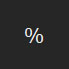
\includegraphics[scale=0.7]{procenta.jpg}
\end{figure}
\end{minipage}
\begin{minipage}{0.45\textwidth}
\begin{itemize}
\item funkce spočítá kolik procent je číslo $x$ ze základu $y$
\item $x$ \keys{\%} $y$ \keys{=}
\end{itemize}
\end{minipage}
\\%log
\begin{minipage}{0.07\textwidth}
\begin{figure}[H]
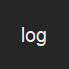
\includegraphics[scale=0.7]{ilog.jpg}
\end{figure}
\end{minipage}
\begin{minipage}{0.45\textwidth}
\begin{itemize}
\item výpočet logaritmu čísla o základu $n$
\item $x$ \keys{log} $n$ \keys{=}
\end{itemize}
\end{minipage}
\begin{minipage}{0.07\textwidth}
\begin{figure}[H]

\includegraphics[scale=0.7]{iln.jpg}
\end{figure}
\end{minipage}
\begin{minipage}{0.45\textwidth}
\begin{itemize}
\item výpočet přirozeného logaritmu čísla
\item \keys{ln} $x$ \keys{=}
\end{itemize}
\end{minipage}
\\%sin
\begin{minipage}{0.07\textwidth}
\begin{figure}[H]
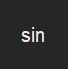
\includegraphics[scale=0.7]{isin.jpg}
\end{figure}
\end{minipage}
\begin{minipage}{0.45\textwidth}
\begin{itemize}
\item výpočet sinu čísla v radiánech
\item \keys{sin} $x$ \keys{=}
\end{itemize}
\end{minipage}
\begin{minipage}{0.07\textwidth}
\begin{figure}[H]
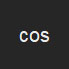
\includegraphics[scale=0.7]{icos.jpg}
\end{figure}
\end{minipage}
\begin{minipage}{0.45\textwidth}
\begin{itemize}
\item výpočet cosinu čísla v radiánech
\item \keys{cos} $x$ \keys{=}
\end{itemize}
\end{minipage}
\\%tan
\begin{minipage}{0.07\textwidth}
\begin{figure}[H]

\includegraphics[scale=0.7]{itan.jpg}
\end{figure}
\end{minipage}
\begin{minipage}{0.45\textwidth}
\begin{itemize}
\item výpočet tangens čísla v radiánech
\item \keys{tan} $x$ \keys{=}
\end{itemize}
\end{minipage}
\newline
\newline
\begin{minipage}{0.07\textwidth}
\begin{figure}[H]

\includegraphics[scale=0.7]{c.png}
\end{figure}
\end{minipage}
\begin{minipage}[t]{0.45\textwidth}
\begin{itemize}
\item vynuluje displej i poslední\\ počítaný příklad
\item \keys{C}
\end{itemize}
\end{minipage}
\begin{minipage}{0.07\textwidth}
\begin{figure}[H]

\includegraphics[scale=0.7]{back.png}
\end{figure}
\end{minipage}
\begin{minipage}[t]{0.7\textwidth}
\begin{itemize}
\item postupně maže číslice na displeji
\item \keys{\backdel}
\end{itemize}
\end{minipage}
\\
\begin{minipage}{0.07\textwidth}
\begin{figure}[H]

\includegraphics[scale=0.7]{otaznik.png}
\end{figure}
\end{minipage}
\begin{minipage}{0.45\textwidth}
\phantom{desdeded}
\begin{itemize}
\item \keys{?} přepnutí do režimu nápovědy
\item kliknutím na tlačítko se zobrazí\\ nápověda
\end{itemize}
\end{minipage}
\begin{minipage}{0.07\textwidth}
\begin{figure}[H]

\includegraphics[scale=0.7]{ans.png}
\end{figure}
\end{minipage}
\begin{minipage}{0.45\textwidth}
\phantom{desdeded}
\begin{itemize}
\item je v něm uložená poslední hodnota
\item \keys{ans}
\end{itemize}
\end{minipage}
\\
\begin{minipage}{0.07\textwidth}
\begin{figure}[H]

\includegraphics[scale=0.7]{m.jpg}
\end{figure}
\end{minipage}
\begin{minipage}[t]{0.9\textwidth}
\begin{itemize}
\item zmáčknutí uloží číslo do paměti (nalevo na displeji se ukáže indikátor \verb M , že je v~paměti uložené číslo)
\item $x$ \keys{M}
\item každé další zmáčknutí \keys{M} zobrazí uložené číslo
\end{itemize}
\end{minipage}
\\
\begin{minipage}{0.07\textwidth}
\begin{figure}[H]

\includegraphics[scale=0.7]{md.jpg}
\end{figure}
\end{minipage}
\begin{minipage}[t]{0.7\textwidth}
\begin{itemize}
\item smaže hodnotu uloženou v paměti (indikátor \verb M \ zmizí)
\item \keys{MD}
\end{itemize}
\end{minipage}
\\%m+
\begin{minipage}{0.07\textwidth}
\begin{figure}[H]
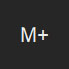
\includegraphics[scale=0.7]{implus.jpg}
\end{figure}
\end{minipage}
\begin{minipage}{1\textwidth}
\begin{itemize}
\item k hodnotě v paměti přičte zadané číslo
\item $x$ \keys{{M+}}
\end{itemize}
\end{minipage}\\
\begin{minipage}{0.07\textwidth}
\begin{figure}[H]

\includegraphics[scale=0.7]{mminus.jpg}
\end{figure}
\end{minipage}
\begin{minipage}{1\textwidth}
\begin{itemize}
\item od hodnoty v paměti odečte zadané číslo
\item $x$ \keys{{M-}} 
\end{itemize}
\end{minipage}
\newline
\section{Převodník měn}
Převede číslo zobrazené na displeji z vybrané výchozí měny na cílovou měnu.
\\%
\begin{minipage}{0.43\textwidth}
\begin{figure}[H]
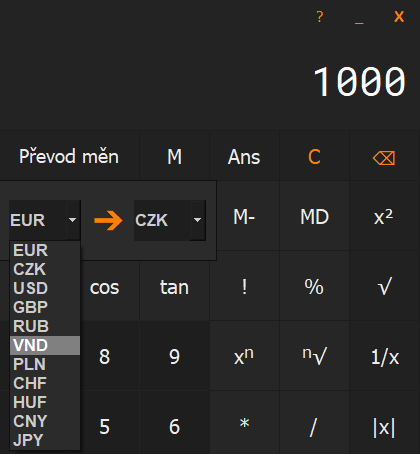
\includegraphics[scale=0.5]{prevodmenrozklik.png}
\end{figure}
\end{minipage}
\begin{minipage}[c]{0.62\textwidth}
\begin{itemize}
\item seznam měn se zobrazí po kliknutí na zkratku měny
\item měnu můžeme vybrat kliknutím nebo se také dá vyhledat pomocí klávesnice (stiknutím prvního písmene zkratky měny), výběr potvrdíme \keys{\return} 

\end{itemize}
\end{minipage}
\\%
\begin{minipage}{0.43\textwidth}
\begin{figure}[H]
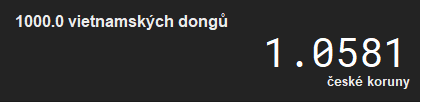
\includegraphics[scale=0.5]{prevedenamena.png}
\end{figure}
\end{minipage}
\begin{minipage}[c]{0.62\textwidth}
\begin{itemize}
\item výpočet se provede kliknutím na \keys{=}\\ nebo stisknutím \keys{\return}
\end{itemize}
\end{minipage}
\end{document}
